\section{Algorithm Compiler}\label{sec:compiler}
\begin{figure}
  \centering
  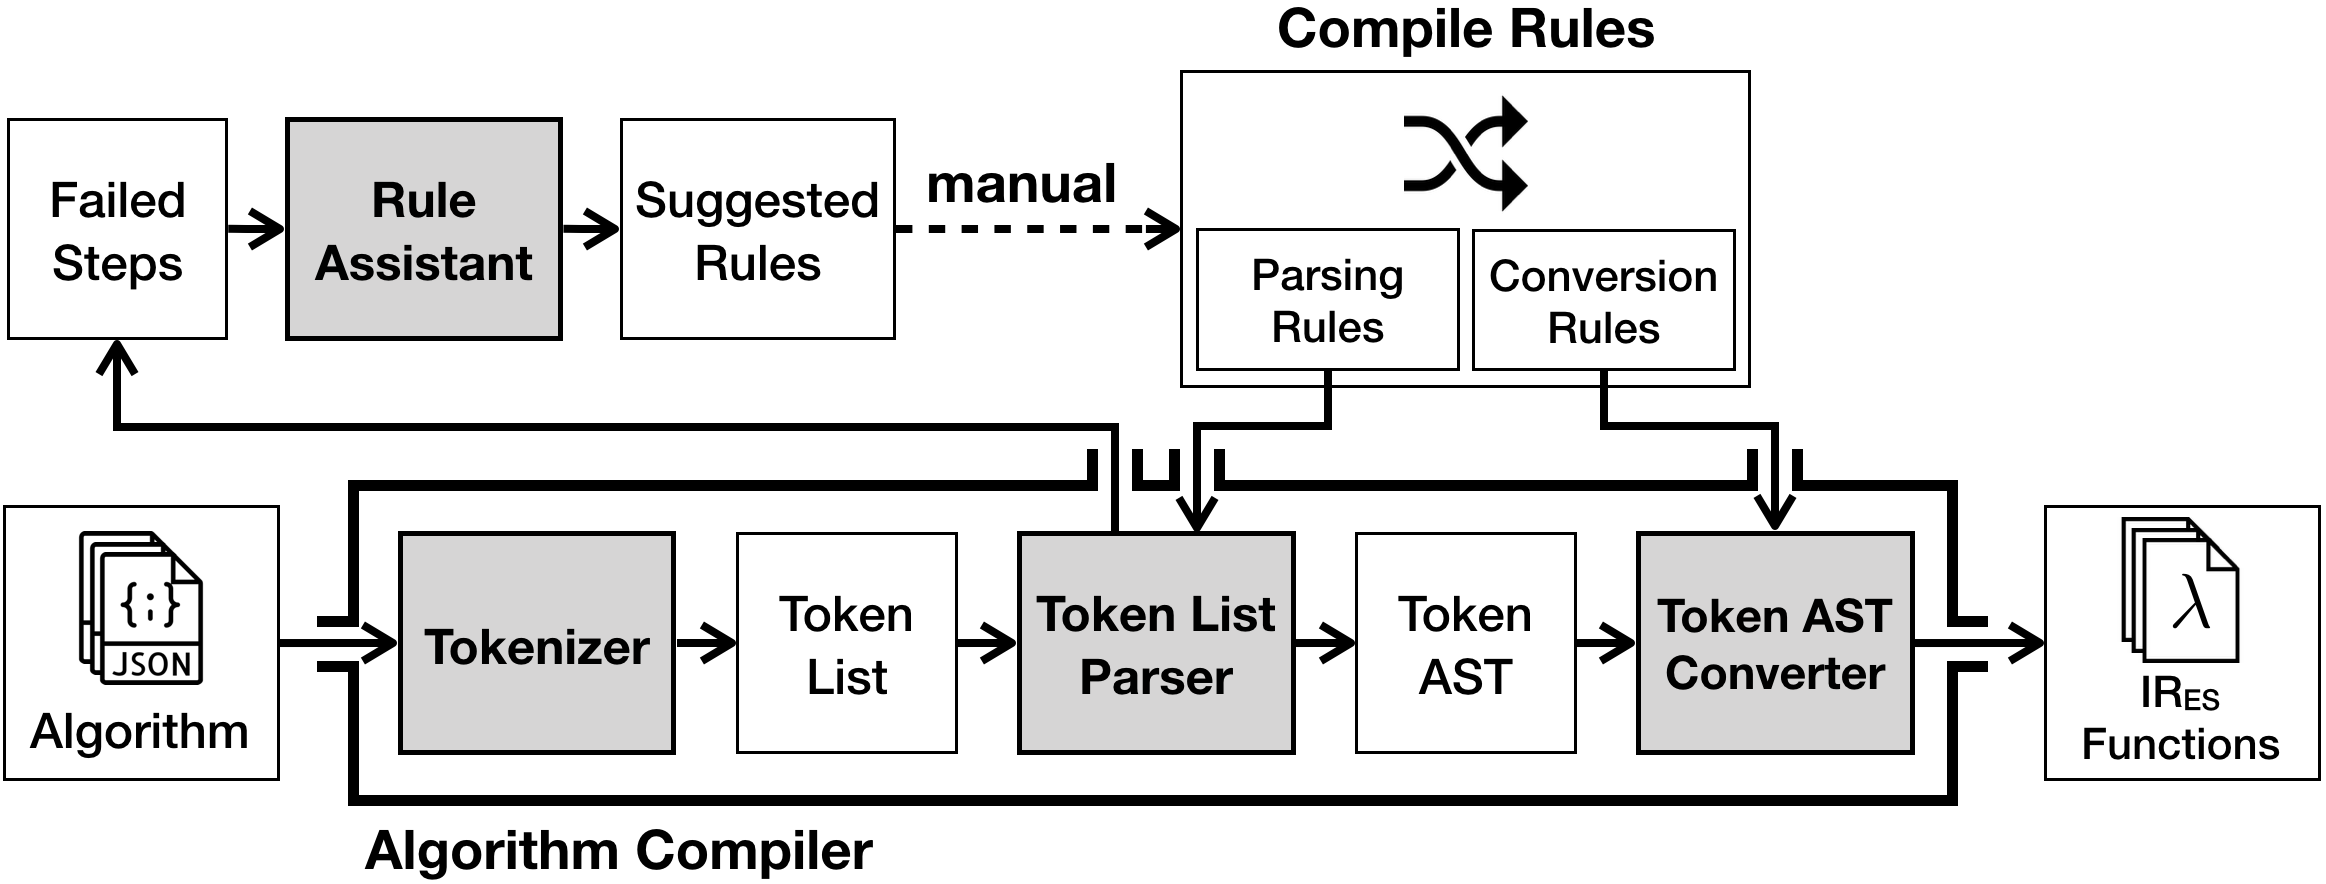
\includegraphics[width=0.5\textwidth]{img/algo_compiler.png}
  \caption{Overall structure of {\sf Algorithm Compiler}}
  \label{fig:algo-compiler}
\end{figure}

In this section, we explain {\sf Algorithm Compiler} that compiles
abstract algorithms to \( \ires \) functions as illustrated in
Figure~\ref{fig:algo-compiler}.

\subsection{Tokenizer}
Before compiling abstract algorithms, {\sf Tokenizer} first tokenizes
each abstract algorithm into a list of tagged tokens.  An algorithm
consists of ordered steps and it may contain sub-steps as well.
For example, the \textbf{\small ToPrimitive} algorithm in
Figure~\ref{fig:to-primitive}(a) has three steps and the second step
has seven sub-steps.  Moreover, the tokens of each step have their own
HTML tags and each tag has a meaning.  For instance, \code{<var>}
denotes variables, \code{<emu-grammar>} denotes productions, and
\code{<code>} denotes ECMAScript code.
% \[
%   \begin{array}{c|l}
%     \text{HTML tags} & \text{meanings}\\\hline\hline
%     \code{<var>} & \text{variables}\\\hline
%     \code{<emu-grammar>} & \text{productions}\\\hline
%     \code{<emu-nt>} & \text{non-terminal syntax}\\\hline
%     \code{<code>} & \text{ECMAScript codes}\\\hline
%     \code{<emu-const>} & \text{constant values}\\\hline
%     \code{<emu-val>} & \text{values}\\\hline
%     \code{<ol>} & \text{ordered sub-steps}\\\hline
%     \code{<ul>} & \text{unordered sub-steps}\\\hline
%     \code{<sup>} & \text{superscripts}\\\hline
%     \text{otherwise} & \text{simple texts}\\\hline
%   \end{array}
% \]
We keep such HTML tag information for each token to generate more precise
{\sf Compile Rules}.  For example, because if and only if a token has
a tag \( \code{<var>} \), it is a parameter or a local variable, we can
construct {\sf Compile Rules} that precisely distinguish identifiers
from other components.

The {\sf Tokenizer} module recognizes the structure of each step,
and divides the step into a sequence of tagged tokens.
If an HTML element has an explicit tag, it is converted to a single token
with the tag.  Otherwise, it is divided into multiple tokens and each token
becomes a sequence of alphanumeric characters or a single non-alphanumeric
character.  For example, in the \textbf{\small ToPrimitive} algorithm,
\( \textbf{\code{"default"}} \) is a single token with the HTML tag \( \code{<code>} \)
and \( \code{@@toPrimitive} \) is divided into three text tokens
\( \code{@} \), \( \code{@} \), and \( \code{toPrimitive} \).

Moreover, {\sf Tokenizer} flattens a structured step to a single token
list to handle multi-step statements easily.  Some statements in
abstract algorithms consist of multiple steps.  For example, the
\( \code{if}\!-\!\code{then}\!-\!\code{else} \) statement often consists of
two steps: one for the \( \code{then} \)-branch and another
for the \( \code{else} \)-branch.  To treat them as a linear structure,
we introduce three special tokens to break down structured algorithms:
\( \tend \) denotes the end of a single step, and \( \tin \) and
\( \tout \) denote the start and the end of nested steps, respectively.
For example, the \textbf{\small ToPrimitive} algorithm is tokenized as follows.
\[
  \begin{array}{l}
    \code{Assert} \cdots \tend\\
    \code{If} \cdots \tin \code{If} \cdots \tend
    \cdots \code{Return} \cdots \tend \tout \tend\\
    \code{Return} \cdots \tend\\
  \end{array}
\]

After tokenizing abstract algorithms, {\sf Algorithm Compiler}
compiles token lists into \( \ires \) functions using
{\sf Token List Parser} and {\sf Token AST Converter}.
They depend on {\sf Compile Rules} and each compile rule
consists of a \textit{parsing rule} and a \textit{conversion rule}:
\begin{lstlisting}[style=myScalastyle]
val CompileRule = ParsingRule ^^ ConversionRule
\end{lstlisting}
For each compile rule, its parsing rule describes how to parse a given
token list into a structured token AST, and its conversion rule describes
how to convert the given token AST structure into an \( \ires \) component.
Now, we explain the token list parser and token AST converter with
parsing rules and conversion rules, respectively.

\subsection{Token List Parser}
Parsing rules determine the token list parser, and each parsing rule
is written in extended Scala parser combinators.  We modified the
meaning of the alternative composition operator ( \( | \) ) to collect
all the longest matched results.  If a parser detects a step that
cannot be parsed with given parsing rules, it reports the step into
{\sf Rule Assistant}.  Even when a parser parses a step successfully,
it also reports the step if it can parse the step in multiple ways.
We use Packrat parsing~\cite{packrat} for parsing rules, which
support left recursion.

We provide two kinds of basic token parsers: tag-based parsers and
content-based parsers.  A tag-based parser just checks whether the next
token has a given tag.  For example, the tag-based parser \( \code{varT} \)
checks whether the next token has the tag \( \code{<var>} \).  A
content-based parser checks whether the next token is a text token and
its content passes a given condition.  For example, the string literal
\( \code{"Let"} \) denotes a content-based parser that checks whether
the next token is a text token with the content \( \code{Let} \).
We also provide two content-based parsers \( \code{word} \) and
\( \code{number} \) that check whether the content of the next token
consists of only alphabets or numbers, respectively.  In parsing
rules, all the helper functions defined in Scala parser combinators
are available.  For instance, the helper function \( \code{repsep(p, q)} \)
generates a new parsing rule that denotes zero or more repetition of the
parsing rule \( \code{p} \) using another parsing rule \( \code{q} \) as
a separator.

Consider the following example parsing rule, which is a simplified
version for the step 2-e-i of the \textbf{ToPrimitive} algorithm.
\begin{lstlisting}[style=myScalastyle]
// statements
val Stmt = "Let" ~ varT ~ "be" ~ Expr ~ "." ^^ ...
val Expr = (          // expressions
  varT ^^ ... |       // identifiers
  "?" ~ Expr ^^ ... | // return if abrupt
                      // function calls
  word ~ "(" ~ repsep(Expr, ",") ~ ")" ^^ ... |
  "<<" ~ repsep(varT, ",") ~ ">>" ^^ ...  // lists
)
\end{lstlisting}
The \( \code{Stmt} \) compile rule describes how to compile statements
with one parsing rule and its conversion rule is omitted for now for
brevity.  The \( \code{Expr} \) compile rule describes how to compile
expressions with four parsing rules.  A token parser with the above
rules parses the step 2-e-i of \textbf{ToPrimitive} to the following
token AST:
\begin{center}
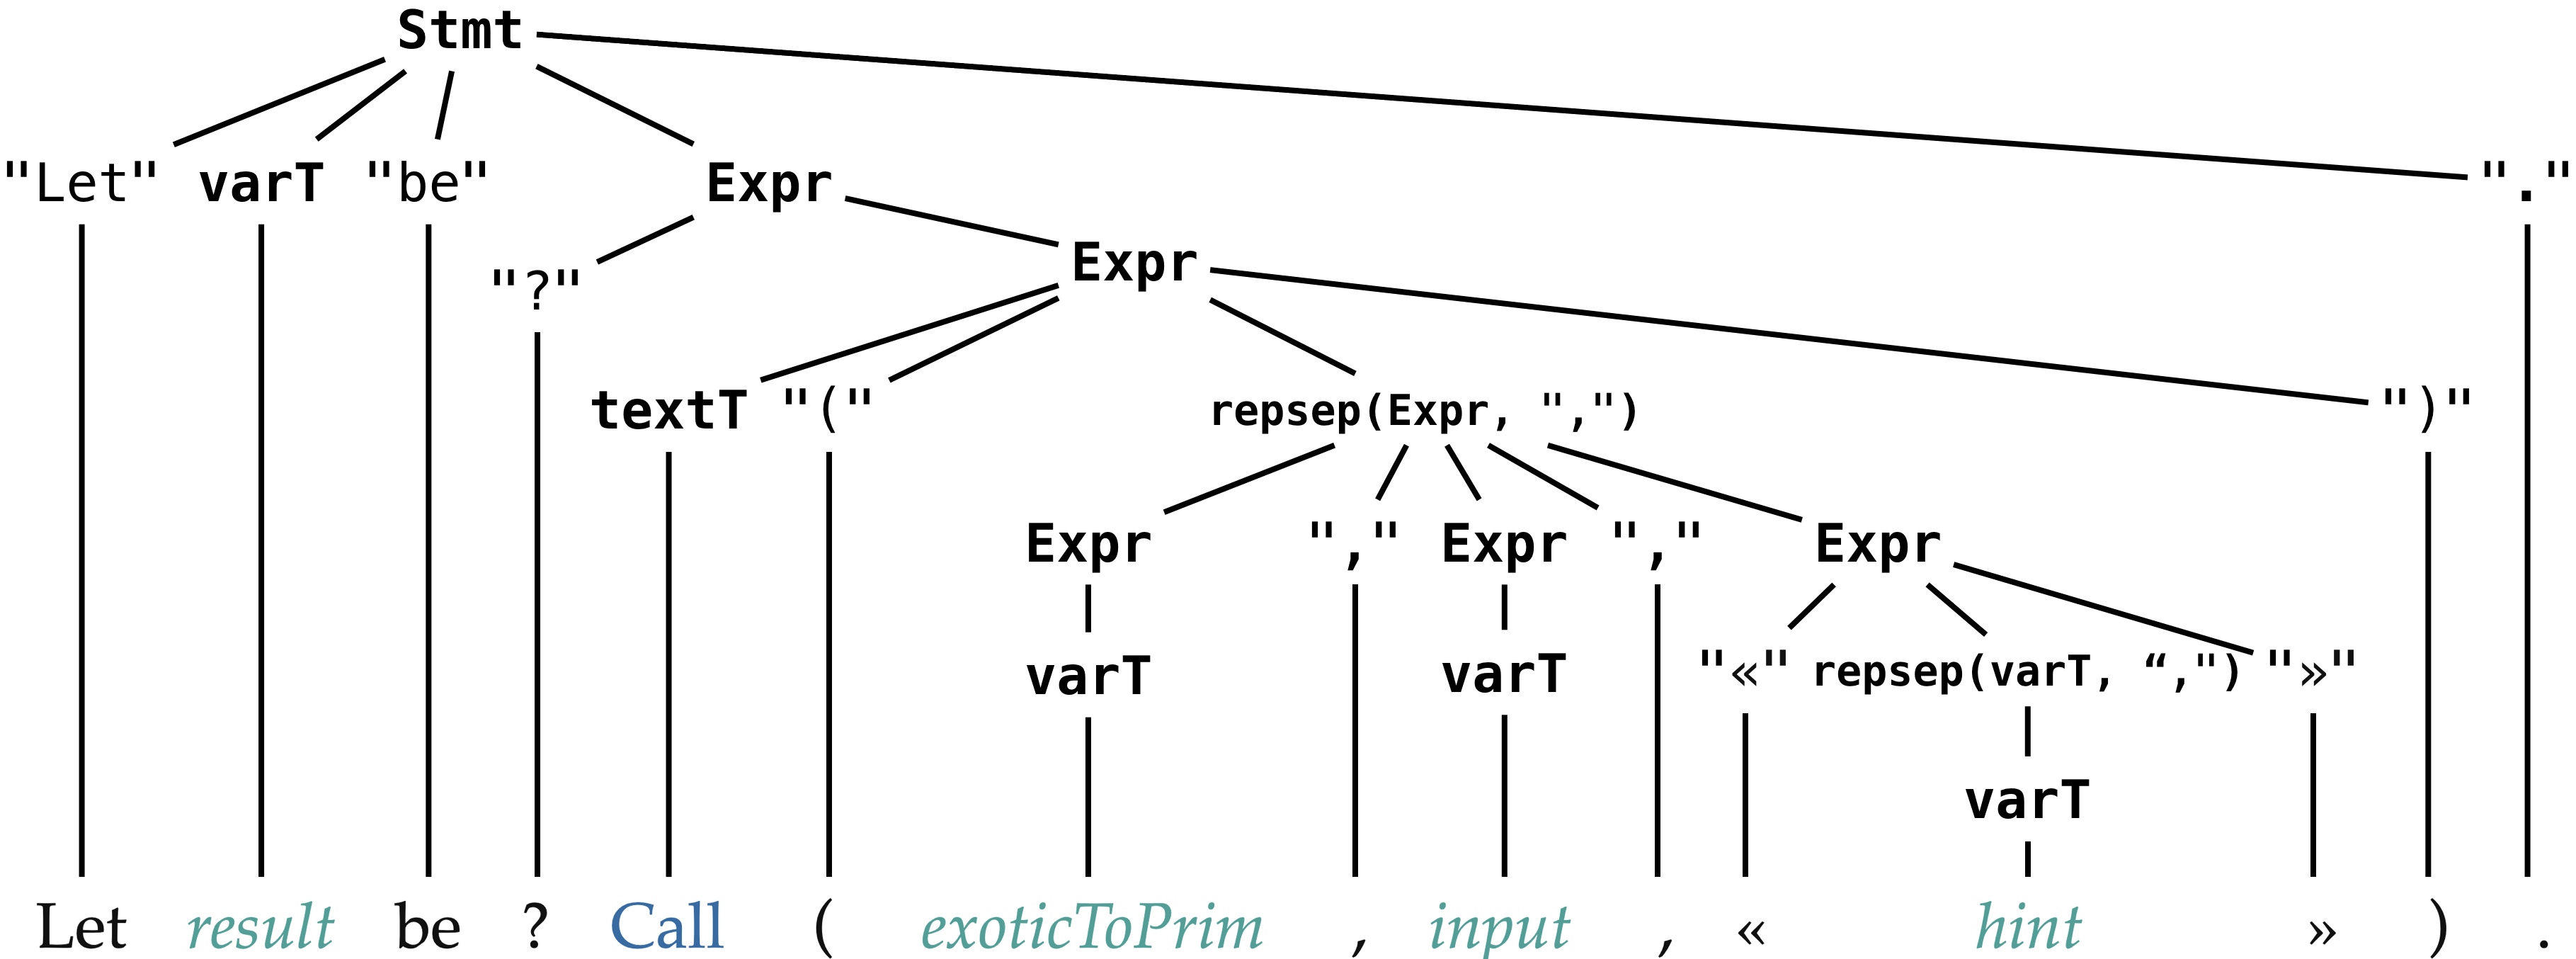
\includegraphics[width=0.5\textwidth]{img/token_ast.png}
\end{center}

\subsection{Token AST Converter}
Conversion rules describe how to generate an \( \ires \) function for a
given token AST.  Each conversion rule is defined with its
corresponding parsing rule.  For basic token parsers, their conversion
rules always return the string values of the contents in parsed tokens.
For example, the following conversion rules are the omitted parts
in the previous example for the step 2-e-i of \textbf{ToPrimitive}:
\begin{lstlisting}[style=myScalastyle]
// statements
val Stmt = ... ^^ { case _ ~ x ~ _ ~ y => ILet(x, y) }
val Expr = (               // expressions
  ... ^^ { x => EId(x) } | // identifiers
                           // return if abrupt
  ... ^^ { _ ~ e => EReturnIfAbrupt(e) } |
                           // function calls
  ... ^^ { case x ~ _ ~ y ~ _ => ECall(x, y) } |
  ... ^^ { case _ ~ x ~ _ => EList(e) } // lists
)
\end{lstlisting}
The conversion rule of the compile rule \( \code{Stmt} \) uses only
the second and fourth sub trees and converts them to \( \ires \)
components.  The second sub-tree is converted to a string value
because it was constructed via the basic token parser \( \code{varT} \).
The fourth sub-tree is converted to an \( \ires \) expression
because the conversion rules of the \( \code{Expr} \) compile rule
construct \( \ires \) expressions.  Then, the conversion rule of
\( \code{Stmt} \) constructs the lexical binding instruction \( \code{ILet} \)
with the string value and the \( \ires \) expression.  In this way,
the step 2-e-i of \textbf{ToPrimitive} is converted to the following
instruction:
\begin{lstlisting}[style=ires]
let result = ? (Call exoticToPrim input (new [hint]))
\end{lstlisting}

We define \( \ires \) to represent abstract algorithms as its
functions with the following design choices:

\begin{itemize}[leftmargin=0.5cm]
\item \textbf{Dynamic typing:} Because each variable in abstract
algorithms is not statically typed, variables do not have their own
static types while each value of \( \ires \) has its dynamic type.

\item \textbf{Imperative style:} \( \ires \) represents algorithm steps
as imperative instructions in the sense that each instruction changes
the current state consisting of an environment and a heap.

\item \textbf{Higher-order functions with restricted scopes:}
In each function of \( \ires \), only global variables, parameters,
and its local variables are available, which means that a function
closure does not capture its current environment.  We use such
restricted scopes because they are enough to represent abstract
algorithms.

\item \textbf{Primitive values:} \( \ires \) supports ECMAScript
primitive values except ``symbols'' because symbols can be represented
as singleton objects.  Also, \( \ires \) provides the unique \(
\code{absent} \) value to represent the absence of parameters.  For
example, when the optional second parameter \( \code{PreferredType} \)
of \textbf{ToPrimitive} in Figure~\ref{fig:to-primitive}(a) is absent,
the parameter has the \( \code{absent} \) value.

\item \textbf{Abstract data types:} \( \ires \) supports only three
abstract data types: \( \code{Record} \) for mappings from some values
to other values, \( \code{List} \) for sequential data, and
\( \code{Singleton} \) for singleton data.  For example, ECMAScript
environment records are represented as \( \code{Record} \)
with string values as keys and addresses as values.  Each key
represents an identifier name and its corresponding address represents
an ECMAScript object.  We also represent constants in the ECMAScript
specification such as \( \code{empty} \) and \( \code{normal} \) as
\( \code{Singleton} \) data types in \( \ires \).
\end{itemize}

\subsection{Rule Assistant}
\begin{algorithm}[t]
  \caption{Fault Localization}\label{alg:fault}
  \begin{algorithmic}[1]
    \Function{FaultLocalize}{$T,n$}\Comment{$T$: failed step, $n$: size}
    \State $S = \varnothing$
    \For{$i = 0$ to $n - 1$}
    \For{$j = i$ to $n - 1$}
    \State $T'$ = a copy of $T$
    \State Substitute $T'[i..j]$ with $\tstar$
    \If{Parse($T'$) contains $\code{Dummy(}x \code{)}$ for some $x$}
    \State Insert $(x, i, j)$ into $S$
    \EndIf
    \EndFor
    \EndFor
    \While{$s = (x, i, j) \in S$}
    \If{$\exists (y, p, q) \in S$ s.t. $i \leq p \wedge q \leq j$}
    \State Remove $s$ from $S$
    \EndIf
    \EndWhile
    \State \Return $S$
    \EndFunction
  \end{algorithmic}
\end{algorithm}

To make it easy to write compile rules, we support a \textit{rule assistant},
which takes not-yet-convertible steps dubbed ``failed steps'' as arguments.
For each failed step, the rule assistant diagnoses a root cause of the
parsing failure.  The basic idea is to check whether we can parse the
failed input with the assumption that a specific sub-sequence of the
failed step is successfully parsed.  We define an approach to find
such sub-sequences of failed steps as \textit{fault localization}.
This approach was actually helpful for us when we update existing
compile rules for new versions of the specification.

The fault localization algorithm is shown in Algorithm~\ref{alg:fault}.
For a given failed step $T$ and the size of a failed input $n$, it
attempts to find a set of the most specific suggestions.  It
substitutes a specific sub-sequence \( T[i..j] \) of \( T \) with the
special token \( \tstar \), which represents some sub-sequence of a
failed step.  It collects a set of possible suggestions, and then
removes more general ones than existing suggestions.  To support this
process, we added a parsing rule  \( \code{starT} \) to each compile
rule as follows:
\begin{lstlisting}[style=myScalastyle]
// statements
val Stmt = ... | starT ^^ { case x => Dummy("Stmt") }
// expressions
val Expr = ... | starT ^^ { case x => Dummy("Expr") }
\end{lstlisting}
where \( \code{starT} \) is a special basic token parser that just
checks whether a given token is the special token \( \tstar \). 
Its corresponding conversion rule is a function that returns a dummy
\( \ires \) component \( \code{Dummy} \) with a string value that
represents the name of its compile rule.

For example, let us assume that the \( \code{Expr} \) compile rule
does not have the alternative for lists:
\begin{lstlisting}[style=myScalastyle]
  "<<" ~ repsep(varT, ",") ~ ">>" ^^
       { case _ ~ x ~ _ => EList(e) } // lists
\end{lstlisting}
Then, the step 2-e-i of \textbf{ToPrimitive} becomes a failed step.
When we use the fault localization algorithm with the failed step and
its size 15, it first finds one suggestion for statements and four
suggestions for expressions as follows:
\[
\footnotesize
\! \! \! \!
  \begin{array}{c}
    (\scode{"Stmt"}, 0, 14), \;
    (\scode{"Expr"}, 3, 13), \;
    (\scode{"Expr"}, 4, 13), \;
    (\scode{"Expr"}, 6, 12), \;
    (\scode{"Expr"}, 10, 12)
  \end{array}
\]
In the \textbf{\small while} loop on lines 9--11, because the last one
is the most specific sub-sequence, it removes the other four
suggestions. Finally, the rule assistant suggests to define another
expression compile rule for the token list \hint{}.
